\documentclass[aspectratio=169]{beamer}

\mode<presentation>
\usetheme{Boadilla}
\definecolor{Columbia}{RGB}{185,217,235}
\definecolor{Columbia2}{RGB}{0,51,160}
\definecolor{Columbia3}{RGB}{0,114,206}
\definecolor{blue}{RGB}{30,90,205}
\definecolor{red}{RGB}{213,94,0}
\definecolor{green}{RGB}{0,128,0}
\setbeamercolor{title}{fg=Columbia3}
\setbeamercolor{frametitle}{fg=Columbia3}
\setbeamercolor{block title}{bg=Columbia3, fg=white}
\setbeamercolor{block body}{bg=white}
\setbeamercolor{structure}{fg=Columbia3}
\setbeamercolor{item projected}{fg=white}
\setbeamercolor{item}{fg=Columbia3}
\setbeamercolor{subitem}{fg=Columbia3}
\setbeamercolor{section in toc}{fg=Columbia3}
\setbeamercolor{description item}{fg=Columbia3}
\setbeamercolor{caption name}{fg=Columbia3}
\setbeamercolor{button}{bg=Columbia3, fg=white}
\usepackage{graphics}
\usepackage{geometry}
\usepackage{booktabs}
\usepackage{tikz}
\usepackage{amsmath}
\usepackage{bbm}
\usetikzlibrary{decorations.pathreplacing}
\usepackage{multirow, makecell}
\usepackage{float}
\usepackage{fancyvrb}
\usepackage{caption}
\usepackage{subcaption}
\usepackage{adjustbox}
\usepackage{threeparttable}
\usepackage{hyperref}
\usepackage[scaled=0.92]{helvet}
\newenvironment{wideitemize}{\itemize\addtolength{\itemsep}{10pt}}{\enditemize}
\newenvironment{wideenumerate}{\enumerate\addtolength{\itemsep}{10pt}}{\endenumerate}
\newenvironment{widedescription}{\description\addtolength{\itemsep}{10pt}}{\enddescription}
\hypersetup{
colorlinks=true,
linkcolor=blue,
filecolor=green, 
urlcolor=blue,
}
\beamertemplatenavigationsymbolsempty
\setbeamercolor{author in head/foot}{bg=white, fg=Columbia3}
\setbeamercolor{title in head/foot}{bg=white, fg=Columbia3}
\setbeamercolor{date in head/foot}{bg=white, fg=Columbia3}
\setbeamercolor{section in head/foot}{bg=white, fg=Columbia3}
\setbeamercolor{page number in head/foot}{bg=white, fg=Columbia3}
\setbeamercolor{headline}{bg=Columbia}
\setbeamertemplate{footline}{
    \leavevmode%
    \hbox{%
        \begin{beamercolorbox}[wd=.333333\paperwidth,ht=2.25ex,dp=1ex,center]{date in head/foot}%
            \usebeamerfont{date in head/foot}\insertshortdate
        \end{beamercolorbox}%
        \begin{beamercolorbox}[wd=.444444\paperwidth,ht=2.25ex,dp=1ex,center]{title in head/foot}%
            \usebeamerfont{title in head/foot}\insertshorttitle
        \end{beamercolorbox}%
        \begin{beamercolorbox}[wd=.222222\paperwidth,ht=2.25ex,dp=1ex, center]{page number in head/foot}%
            \usebeamerfont{page number in head/foot} \insertframenumber{} / \inserttotalframenumber
        \end{beamercolorbox}}%
        \vskip0pt%
    }
%\setbeamercolor{page number in head/foot}{fg=black}
\setbeamertemplate{section in toc}[sections numbered]
\setbeamertemplate{subsection in toc}{\leavevmode\leftskip=3em\rlap{\hskip-1.75em\inserttocsectionnumber.\inserttocsubsectionnumber}\inserttocsubsection\par}
\setbeamerfont{subsection in toc}{size=\footnotesize}
%\setbeamertemplate{headline}{%
  %\begin{beamercolorbox}[ht=5.5ex]{section in head/foot}
    %\vskip2pt\insertnavigation{0.33\paperwidth}\vskip2pt
  %\end{beamercolorbox}%
%}
\newenvironment{transitionframe}{\setbeamercolor{background canvas}{bg=Columbia3}\setbeamertemplate{footline}{} \begin{frame}}{\end{frame}}


\makeatletter
\let\@@magyar@captionfix\relax
\makeatother


\title[Recitation 9]{Recitation 9} % Change this regularly
\author[Seung-hun Lee]{Seung-hun Lee}
\institute[Columbia University]{Columbia University}

\date[December 6th, 2021]{December 6th, 2021}

\begin{document}
\begin{frame}
\titlepage
\end{frame}

\begin{frame}
\frametitle{Experiments in Economics}
\begin{itemize}
\item You categorize some individuals under treatment group and controlled group and compare the differences across groups and times. 
\item You can do this in lab setting (randomized control trials) or find an exogenous event (natural experiments) which derives cross-sectional and time variation
\item They provide a conceptual benchmark for assessing observational studies and can solve many validity threats in regular regressions.
\item Do note that they have a validity threat of their own
\item Further discussion of related topics - potential outcome frameworks, average treatment effect etc - are in the notes
\end{itemize}
\end{frame}


\begin{frame}
\frametitle{Difference in Differences: Regression format}
\begin{itemize}
\item Assume two time periods (before and after) and two groups (treated and controlled)
\item You have the following regression
\[
Y_{it} = \beta_0 + \beta_1 X_{it} + \beta_2 D_{it} + \beta_3 X_{it}D_{it}+u_{it}
\]
where $X=1$ if in treatment, $D=1$ if after treatment
\item You can get the following group averages
\begin{itemize}
\item Treated, After: $E[Y_{it}|X_{it}=1, D_{it}=1] = \beta_0+\beta_1 + \beta_2 + \beta_3$
\item Treated, Before: $E[Y_{it}|X_{it}=1, D_{it}=0] =\beta_0+ \beta_1 $ 
\item Controlled, After: $E[Y_{it}|X_{it}=0, D_{it}=1] =\beta_0+ \beta_2 $
\item Controlled, Before: $E[Y_{it}|X_{it}=0, D_{it}=1] =\beta_0 $ 
\end{itemize}
\item Difference-in-differences  $\hat{\beta}^{DD}=[\bar{Y}_{\text{treat,after}}-\bar{Y}_{\text{treat,before}}]-[\bar{Y}_{\text{control,after}}-\bar{Y}_{\text{control,before}}]$
\begin{itemize}
\item In the above equation, we would be looking at $\hat{\beta}_3$
\end{itemize}
\item Can be generalized to many time periods and many groups with TWFE, Event-studies etc (active area of research)
\end{itemize}
\end{frame}

\begin{frame}
\frametitle{Difference in Differences: In pictures}
\begin{figure}[H]
\centering 
\caption{DD estimator}
\begin{subfigure}[b]{.45\textwidth}
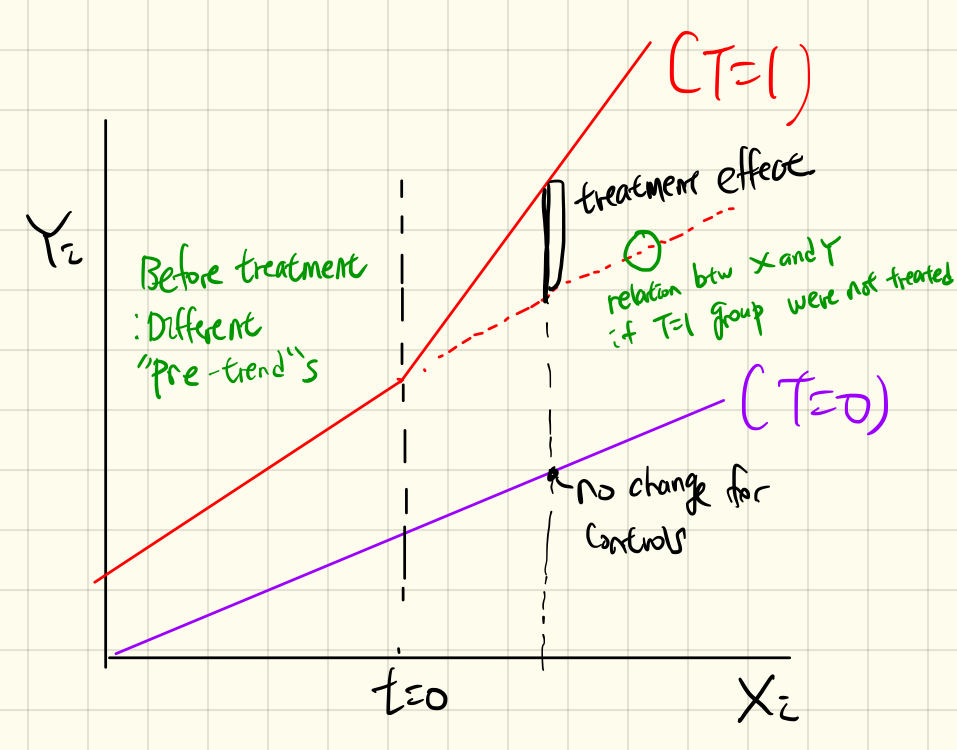
\includegraphics[width=\textwidth]{fig1_1.png}
\caption{No change in control group}
\end{subfigure}
\begin{subfigure}[b]{.45\textwidth}
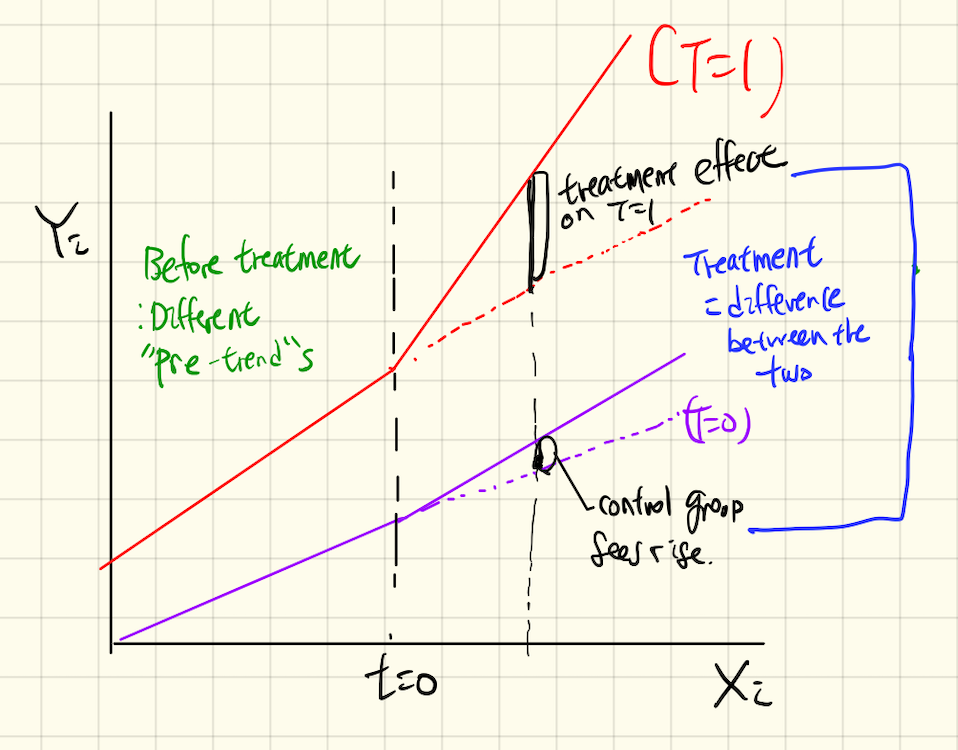
\includegraphics[width=\textwidth]{fig1_2.png}
\caption{Some change in control group}
\end{subfigure}
\end{figure}
\end{frame}


\begin{frame}
\frametitle{Big data}
\begin{itemize}
\item It can simply mean data with large observations or large number of control variables. 
\item In general instances, atypical data such as text data, and satellite imagery are referred to as big data. 
\item In this class, we focus on the instance where there are many control variables, specifically on what to do if there are many control variables relative to the number of observations. 
\item Additionally, we focus on trying to get the best way to predict a result that is currently not in the dataset.
\end{itemize}
\end{frame}

\begin{frame}
\frametitle{Characterizing MSPE}
\begin{itemize}
\item Regression format is 
\[
Y_{i}^*=\beta_1X_{1i}^*+....+\beta_kX_{ki}^*+u_i^*
\]
\item  $X_{1i}^*$ is the ``standardized" version of $X_{1i}$'s, $Y^*_i$ the ``demeaned" version.
\item  Note that we CANNOT have a constant term $\beta_0$ here because if we demean $\beta_0$, which is the same for all $i$'s, they vanish. 
\item MSPE:  the expected value of the squared error made by predicting $Y$ for an observation not in the dataset.
\[
MSPE= E[Y^{OS}-\hat{Y}^{OS}]^2
\]
\begin{itemize}
\item $\hat{Y}^{OS}$: obtained from the coefficients of $\beta$'s made from the in-sample
\item $Y^{OS}$ : realized value of $Y$ outside of the sample
\end{itemize}
\end{itemize}
\end{frame}

\begin{frame}
\frametitle{Characterizing MSPE}
\begin{itemize}
\item With these notations, we can define the prediction error as
\[
Y_i^{OS}-\hat{Y}_i^{OS}=(\beta_1-\hat{\beta}_1)X^{OS}_{1i}+...+(\beta_k-\hat{\beta}_k)X^{OS}_{ki}+u_i^{OS}
\]
\item Define $\sigma_u^2=E[u_i^{OS}]^2$, then we can write MSPE as
\[
MSPE=\sigma_u^2+ E[(\beta_1-\hat{\beta}_1)X^{OS}_{1i}+...+(\beta_k-\hat{\beta}_k)X^{OS}_{ki}]
\]
\item Oracle prediction: the smallest possible MSPE, $\sigma_u^2$
\item However,  we cannot predict $\beta$'s perfectly.
\item The more predictors we have, we generally end up having larger MSPE $\to$ need to reduce $X$'s. 
\item Need Ridge, LASSO, and Principal Component method comes in

\end{itemize}
\end{frame}


\begin{frame}
\frametitle{Methods}
\begin{itemize}
\item Goal: Find other estimators that does not increase the MSPE compared to the rate in which the same rises in OLS estimators. 
\item Idea: Reduce the $\sigma_u^2$, the variance from the residual sums of squares, at the expense of introducing a small bit of bias. 
\item How: Providing a penalty for having a model with large number of regressors (what we formally call `shrinkage'). 
\end{itemize}
\end{frame}

\begin{frame}
\frametitle{Ridge}
\begin{itemize}
\item Minimize a `penalized' sum squared of residuals
\[
\hat{\beta}_{Ridge}=\arg\min_{\beta_1,..,\beta_k}\left[ \sum_{i=1}^n(Y_i - \beta_1X_{1i}-....-\beta_kX_{ki})^2 + \lambda_{Ridge}\sum_{j=1}^k\beta_j^2\right]
\]
\item $\lambda_{Ridge}\sum_{j=1}^k\beta_j^2$: penalty for complexity. 
\item Introduce bias so that the variance term $\sigma_u^2$ will be reduced.
\item Variance and the bias in MSPE moves in a trade-off relation 
\item Ridge estimator minimizes MSPE by reducing the variance term to the extent that the bias term does not rise too drastically. 
\end{itemize}
\end{frame}

\begin{frame}
\frametitle{LASSO}
\begin{itemize}
\item Penalty term takes a different form: 
\[
\hat{\beta}_{LASSO}=\arg\min_{\beta_1,...,\beta_k}\left[ \sum_{i=1}^n(Y_i - \beta_1X_{1i}-....-\beta_kX_{ki})^2 + \lambda_{LASSO}\sum_{j=1}^k |\beta_j|\right]
\]
\item The difference between the two lies in the degree of shrinkage. 
\begin{itemize}
\item When the OLS estimates are small, the LASSO shrinks those estimates all the way to 0. 
\item Ridge also shrinks those coefficients close to 0, they do not exactly set them to 0. 
\end{itemize}
\end{itemize}
\end{frame}

\begin{frame}
\frametitle{Principal component}
\begin{itemize}
\item You are using a linear combination of some subset of $k$ variables so that you end up with $p<k$ number of regressors (`collapsing' the model)
\item Solve the following problem to get the $j$'th principal component $PC_j$
\[
\max var\left(\sum_{i=1}^Ka_{ji}X_i\right)\  \text{s.t.}\ \sum_{i=1}^ka_{ji}^2=1
\]
with another condition being that $corr(PC_j,PC_{j-1})=0$
\item Solve the \textit{maximization}: We want the $X$'s to explain more of the variation
\item $\sum_{i=1}^ka_{ji}^2=1$: Regularization method
\item $corr(PC_j,PC_{j-1})=0$: We want to minimize the overlapping amount of information across different principal components.
\end{itemize}
\end{frame}
%%%%%%%%%%%%% Section 1. 
%%%%%%%%%%%
\end{document}
